Suppose one day you meet a biologist you want to impress and she tells you all about her four favorite species of orchids that she has been studying for years. In order to figure out the ancestral relationships among them and draw a phylogenetic tree (a diagram biologists use to show these evolutionary relationships), she has been chasing them around the mountains, took many DNA samples, later sat behind her computer, aligned them, and did many other things biologists do to arrive to their phylogenetic trees. But no matter how much she tried to eliminate any errors on her side, she kept getting two different phylogenetic trees, both equally likely. Finally she started suspecting a hybridization event took place during the evolution of these four species. Now she simply doesn't know how to represent that in a single tree. 

This is a valid scenario and it might happen to you any time. In this thesis we will try to help you impress a biologist of your choice. 

So let's look at her trees ($T_1$ and $T_2$ in figure \ref{fig:toyex}). She marked her orchid species by black circles and labeled them $a,b,c,d$. The hypothetical ancestors she marked by black squares. One tree suggests that long time ago these orchids split into two lineages; from one later species $a$ and $b$ differentiated, and from the other, species $c$ and $d$. The second tree paints a very different picture of what happened. It suggests that species $a$ was the first one to split off from the common ancestor of all four of them. After that event, species $d$ split off. Finally $b$ and $c$ differentiated as well. 

  %-----------------------------------------------------------------------------
  \begin{figure}[h]
    \centering
    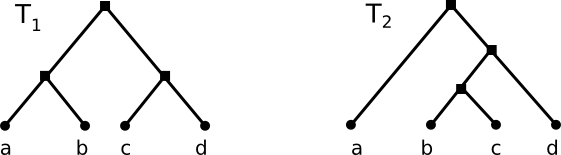
\includegraphics[scale=0.5]{../figs/ch1/toyex.png}
    \caption{Two conflicting evolutionary histories for four species $a,b,c$ and $d$}
    \label{fig:toyex}
  \end{figure}
  %-----------------------------------------------------------------------------

As a computer scientist or a mathematician you understand that no tree can represent all these events at the same time. You will need something more general than a tree, a directed acyclic graph, which we will here often call a network. So you draw two networks ($N_1$ and $N_2$ in figure \ref{fig:toyex1}) on four species (which you keep calling leaves instead of flowers much to her dismay). You explain why $N_1$ contains both trees $T_1$ and $T_2$ (in figure \ref{fig:toyex2}) and that the same argument holds for $N_2$.  You interpret $N_1$ as follows: first species $a$ differentiated from the common ancestor of all four orchids. Then $d$ split off, after that $c$. Finally, ancestors of $a$ and $c$ exchanged their genetic material and formed a hybrid species $b$. This is why species $b$ seems genetically closest to $a$ in $T_1$ and to $c$ in $T_2$. A single tree simply cannot represent all that happened. Multiple trees or a network that summarizes them tell the full story. 

You start interpreting $N_2$ when she interrupts you and says that it is unlikely $N_2$ happened according to Occam's razor, since it assumes more hybridization events than $N_1$ while explaining the same situation.

  %-----------------------------------------------------------------------------
  \begin{figure}[h]
    \centering
    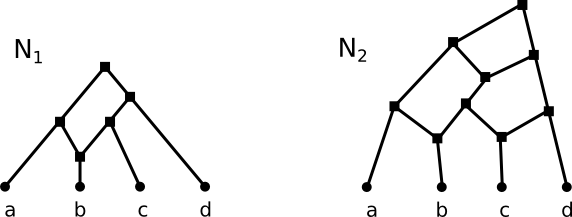
\includegraphics[scale=0.5]{../figs/ch1/toyex2.png}
    \caption{Two nontree-like (hypothetical) evolutionary histories, each of which contains both tree-like histories $T_1$ and $T_2$ at the same time.}
    \label{fig:toyex1}
  \end{figure}
  
    \begin{figure}[h]
    \centering
    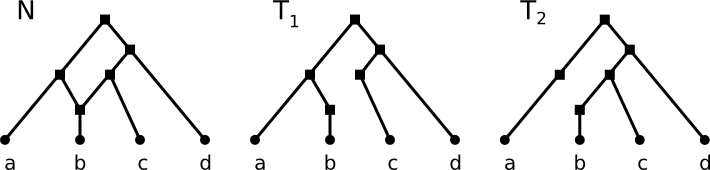
\includegraphics[scale=0.5]{../figs/ch1/toyex1.png}
    \caption{How removing appropriate edges of $N_1$ leads to either $T_1$ or $T_2$.}
    \label{fig:toyex2}
  \end{figure}
  %-----------------------------------------------------------------------------

You know enough. You understand this is a combinatorial problem and you have a good idea of which parameter you need to minimize. You are interested in finding a network that contains all input trees and has a minimum number of hybridization events, or nodes with more than one incoming edge. 
% a ``friendlier'' alternative
%\textcolor{magenta}{A ``friendlier'' alternative for the above paragraph: Biologists have been able to piece together a great deal of information concerning the tree of life -- relying in particular in more recent time on the advent of even cheaper and faster DNA sequencing technologies. Even so, there remain many fascinating open problems concerning the tree of life and the evolutionary process underlying it, problems that often require sophisticated techniques from areas such as mathematics, computer science and statistics.}
Solving this problem requires searching for an optimal network across a vast space of possible networks. Since there are only finitely many such networks, one might think it is plausible (for a computer) to consider every single network and pick the best one, according to some measure of best. This approach is called exhaustive search and the problem with it is in its dependency on the number of the species we are considering. The bigger the number of species in a tree, the bigger the space of possible networks (and thus bigger the amount of time we need to solve the problem). 
In fact only a small increase in the size of the input trees leads to an exponentially big increase in the search space. The number of leaf-labeled rooted trees has been known since 1870 from classical work of Scr\"{o}der \cite{countingtrees}, while the number of leaf-labeled rooted networks was counted recently in \cite{countingdags}.


Ideally, we are interested in algorithms that don't depend this much on the varying size of the input, in the same way that adding two very big numbers is not much harder than adding two small ones. The question is, is it even possible to find such an algorithm for combining two trees into a network? 

Complexity theory is a branch of mathematics that gives us a framework for classifying algorithmic problems according to their computational hardness. It distinguishes between two big classes of problems that are believed (but not proven) to be different, P and NP. 




{
Officially these classes are defined with respect to decision problems, i.e. problems that are defined as a question about existence of a solution. A solution to such a problem is a correct ``yes'' or ``no'' statement. The class of ``easy'' or polynomially solvable problems, P, is a class of decision problems for which an efficient algorithm exists, i.e. one that runs in time that is bounded by some polynomial function of the size of an instance. We say that a decision problem is in class NP, class of nondeterministically polynomially solvable problems, if for a ``yes''-answer a certificate can be given that can be verified within a running time bounded by a polynomial function of the input size. The class of hardest problems, called NP-hard, contains decision problems that have an additional property: a solution of just one of these problems in polynomial time would imply solution of any other problem in NP in polynomial time. When a problem is both NP-hard and in NP we say that it is NP-complete. So problems in P are the easiest problems in NP, while the hardest problems in NP are NP-complete. 
}

{
The toy problem we have just encountered was not formulated as a decision problem but an optimization problem \footnote{To be more precise, the toy problem as we initially defined it is a construction one because we asked for a \textit{network} with fewest reticulations, not just the minimum \textit{number} of reticulations. But for now lets concentrate on its optimization variant, because we are not discussing complexity of that particular problem, we simply want to introduce some definitions.}, i.e. it asks for an optimum solution (fewest hybridization events) out of many possible ones. But any optimization problem has a decision version. In our case, instead of asking for a rooted network that contains two input trees and has a minimum number of ``non-tree-like'' nodes (vertices of in-degree higher than 1), we could chose a constant $k$ and ask ``does there exist a network that contains two input trees and has at most $k$ non-tree-like nodes. These two formulations of the problem are equivalent because if we could solve the decision version in polynomial time, then we could (using binary search) solve the optimization version in polynomial time (and obviously if we could solve the optimization version in polynomial time we could solve the decision version in polynomial time as well).  


Like many computational problems in life sciences or operations research, the problem of combining two trees into a network the way we described above, is NP-hard. The next question is of course what can be done to solve an NP-hard problem in practice. There are numerous standard approaches, but here we will encounter two of them: approximation and parameterized complexity. 



%-----------------approximation-------------------------------
Almost as soon as the concept of NP-hardness was introduced, people asked themselves if instead of finding an optimal solution to a minimization problem we can find, in polynomial time, a solution that is within a factor $(1+ \epsilon)$ of an optimum for some $\epsilon >0$ (or within a factor $(1 - \epsilon)$ if we are dealing with a maximization problem). Furthermore, we would like $(1+\epsilon)$, also called approximation ratio, to be some constant rather than a function that depends on the input size of the problem. In that case we say a problem is in APX, the class of NP-hard problems for which polynomial time approximation algorithm exists that can achieve a constant worst-case approximation ratio. 

{
Similarly to class NP we can define a class of APX-hard and APX-complete problems, which are seen as ``difficult'' approximation problems. If there is a polynomial-time algorithm to solve a problem to within \emph{every} multiplicative factor of the optimum other than 1, then the problem is said to have a polynomial-time approximation scheme (PTAS). A problem is said to be APX-hard if there is a PTAS reduction (a reduction that preserves the property that a problem has a PTAS) from every problem in APX to that problem, and to be APX-complete if the problem is APX-hard and also in APX. 
}



%-----------------parametrized--------------------------------
Sometimes however, it is not desirable to have an approximation algorithm. As we already saw, if a biologist is looking for a network to explain what exactly happened in the evolution of a small number of species, then giving as a solution a network from figure \ref{fig:toyex1} on the right is unsatisfying, as it depicts a wrong picture of the reality if we stick to the principle of Occam's razor. In that case we want efficient exact algorithms and the key word here is parameterized complexity. 

The idea is to design an algorithm for a hard problem that runs in polynomial time with respect to the size of the instance, but exponential in the value of some chosen parameter. %The point here is that we are looking for a parameter that somehow partitions the set of all input instances. 
For example, such an algorithm can have time complexity $c^k poly(n)$, where $c$ is some constant, $n$ is the input size and $k$ is the value of a parameter of the given input. For a small $k$ this algorithm can be considered to be efficient. When such an algorithm exists, we say the problem is in FPT. See \cite{downey1999,niedermeier2006} for an introduction to fixed parameter tractability.


For a book on complexity theory we refer a reader to \cite{Arora}. Throughout the thesis we will assume the reader to be familiar with (very) basic graph theory; for a reference to basic graph theory see \cite{diestel2000graph}. 


\section{Definitions}
  %------------------------------------------------------------------------------
  \subsection*{Phylogenetic trees}

As we have already seen in that simple example of interaction between a biologist and a mathematician in the beginning of this chapter, the evolutionary history of a set of contemporary species is often modeled as a \emph{rooted phylogenetic tree}. Essentially, this is a rooted tree in which the leaves are bijectively labeled by the set of species and edges are directed away from the root, reflecting the direction of evolution \cite{SempleSteel2000}. Furthermore, the root represents the common ancestor of the set of species the tree is modeling and nodes of outdegree two or higher model the points in history at which a common ancestor of a subset of the species differentiated into two or more sublineages. The central problem in phylogenetics is to recover the topology of the ``true'' phylogenetic tree, given only information about the species, often DNA data. This is a challenging computational problem and has been the topic of intensive research during the last 40 years \cite{MathEvPhyl,reconstructingevolution,SemSte03}. 


Without further ado, denote the set of species (or more generally, \emph{taxa}) by $X$. A \emph{rooted phylogenetic $X$-tree $T$} is a rooted tree with no nodes with indegree~1 and outdegree~1, a root with indegree 0 and outdegree 2, and leaves bijectively labeled by the elements of $X$. Such a tree is called \emph{binary} if all inner nodes except the root have indegree~1 and outdegree~2. When some nodes have outdegree higher than 2, we speak of \textit{nonbinary} trees. We will encounter nonbinary trees in Chapter \ref{ch:3} and we postpone definitions of nonbinary concepts until then. For now we only talk of binary setting and we will refer to a rooted binary phylogenetic $X$-tree as a \emph{tree} for short. The edges of any rooted tree should be seen as being directed away from the root even though we will commonly draw them instead of arcs.

  %-----------------------------------------------------------------------------
  \begin{figure}[t]
    \centering
     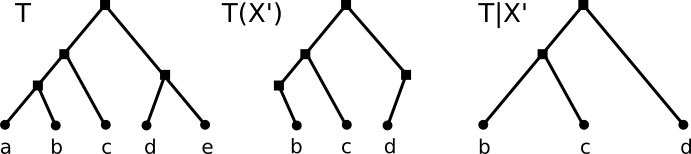
\includegraphics[width=0.7 \textwidth]{../figs/ch1/introtree.png}
    \caption{Let $X$ be a set of taxa $\{a,b,c,d,e\}$ and $X'$ its subset $\{b,c,d\}$. This figure shows an $X$-tree $T$, a minimal subtree of $T$ on $X'$ and a restriction of $T$ to $X'$.}
    \label{fig:introtree}
  \end{figure}
  %-----------------------------------------------------------------------------


The set of leaves of~$T$ is denoted as~$\cL(T)$. We identify each leaf with its label. In the course of this thesis, different types of subtrees play an important role. Let~$T$ be a rooted phylogenetic $X$-tree and~$X'$ a subset of~{$\cL(T)$}. The minimal rooted subtree of~$T$ that connects all leaves in~$X'$ is denoted by $T(X')$. Furthermore, the tree obtained from $T(X')$ by suppressing all {vertices with indegree and outdegree both equal to 1} is the {\it restriction of $T$ to $X'$} and is denoted by $T|X'$. See Figure \ref{fig:introtree}.

Let~$T$ be a rooted phylogenetic $X$-tree and~$S$ a rooted phylogenetic $X'$-tree for some $X' \subseteq X$. We say that~$S$ is a \emph{pendant subtree} of~$T$ if it is a subtree that can be detached from~$T$ by deleting a single edge. For a set~$\T$ of phylogenetic $X$-trees and $X' \subseteq X$, a \emph{common pendant subtree} of~$\T$ is a rooted phylogenetic $X'$-tree that is a pendant subtree of each tree in~$\T$. 

{
For $n\geq 2$, an {\it $n$-chain} of $T$ is an $n$-tuple $(a_1,a_2,\ldots,a_n)$ of elements of $\cL(T)$ such that the parent of $a_1$ is either the same as the parent of $a_2$ (see Figure \ref{fig:chains_ex} left) or the parent of $a_1$ is a child of the parent of $a_2$ (see Figure \ref{fig:chains_ex} right) and, for each $i\in\{2,3,\ldots,n-1\}$, the parent of $a_i$ is a child of the parent of $a_{i+1}$. The subgraph induced by $a_1,a_2,\ldots,a_n$ and their parents is called a {\em caterpillar}.
A \emph{common chain} of a set~$\T$ of trees is a maximal tuple $(x_1, x_2,...,x_q)$ that is a chain of each tree in~$\T$.
}

\begin{figure}[h]
 \centering
 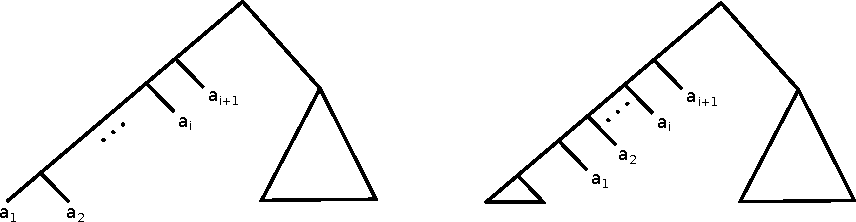
\includegraphics[width=0.9 \textwidth]{../figs/ch1/chains.pdf}
 \caption{Example of $n$-chains}
 \label{fig:chains_ex}
\end{figure}


However, our understanding of evolutionary mechanisms has deepened and there is growing awareness that evolution is not always treelike \cite{expanding}. In particular, due to \emph{reticulate phenomena} such as hybridizations, recombinations and horizontal gene transfer the evolution of a set of species is sometimes better modeled as a network rather than a tree \cite{davidbook}. Trees remain still equally relevant and they are often used as building blocks for networks.


\subsection*{Hybridization networks}
A \emph{rooted phylogenetic network} is essentially a generalisation of phylogenetic trees to directed acyclic graphs (DAGs). In such graphs nodes with indegree two or higher, known as \emph{reticulations}, represent the points at which two or more lineages merge, rather than diversify. 

Formally, a {\it rooted phylogenetic network $N$} on a set~$X$ is a rooted acyclic directed graph, which has a single root of outdegree 2, has no vertices with indegree and outdegree both~1, and in which the vertices of outdegree~0 are bijectively labelled by the elements of~$X$. A phylogenetic network is \emph{binary} if all vertices have indegree and outdegree at most~2 and every vertex with indegree~2 has outdegree~1. Intuitively we say that a phylogenetic network $N$ \emph{displays} a phylogenetic tree $T$ when all of the ancestral relationships visualized by~$T$ are visualized by~$N$. A precise definition will be given shortly. 

Following the publication of several seminal articles in 2004-5 (e.g. \cite{baroni05,BaroniEtAl2004}) there has been considerable research interest in the biologically-inspired question from the beginning of this chapter. Namely, given two rooted phylogenetic trees $T_1$ and $T_2$ on the same set of taxa $X$, what is the minimum number of reticulations required by a phylogenetic network $N$ on $X$ which displays both $T_1$ and $T_2$? This value is often called the \emph{hybridization number} in the literature, and when addressing this specific problem the term \emph{hybridization network} is often used instead of the more general term phylogenetic network. For the purpose of consistency we will henceforth use the term hybridization network. We now list some necessary definitions. 

For each vertex~$v$ of $N$, we denote by $d^-(v)$ and $d^+(v)$ its indegree and outdegree respectively. If $(u,v)$ is an arc of $N$, we say that~$u$ is a \emph{parent} of~$v$ and that~$v$ is a \emph{child} of~$u$. Furthermore, if there is a directed path from a vertex~$u$ to a vertex~$v$, we say that~$u$ is an \emph{ancestor} of~$v$ and that~$v$ is a \emph{descendant} of~$u$.

A vertex of indegree greater than one represents an evolutionary event in which lineages combined, such as a hybridization, recombination or horizontal gene transfer. We call these vertices \emph{hybridization vertices}. To quantify the number of hybridization events, the {hybridization number} of a (nonbinary) hybridization network $N$ is given by
$$h(N)=\sum_{v}(d^-(v)-1)$$
where $v$ goes over all vertices of $N$ except the root.
In a binary network, $h(N)$ is simply the number of vertices with indegree 2. Observe that $h(N)=0$ if and only if~$N$ is a tree.

Let $N$ be a hybridization network on~$X$ and~$T$ a rooted binary phylogenetic $X'$-tree with $X'\subseteq X$. We say that~$T$ is {\it displayed} by~$N$ if~$T$ can be obtained from~$N$ by deleting vertices and edges and suppressing vertices with $d^+(v)=d^-(v)=1$ (or, in graph-theoretic words, if a subdivision of~$T$ is a subgraph of~$N$). 

The problem {\sc MinimumHybridization}, abbreviated \mh, is to compute the {hybridization number} of two rooted binary phylogenetic $X$-trees~$T_1$ and~$T_2$, which is defined as
$$h(T_1,T_2)=\min\{h(N): N \mbox{ is a hybridization network that displays } T_1 \mbox{ and }T_2\},$$
i.e., the minimum number of hybridization events necessary to display two rooted binary phylogenetic trees.

This problem can be formulated as an optimization problem in the obvious way.\\

\noindent{\bf Problem:} {\sc MinimumHybridization}\\
\noindent {\bf Instance:} Two rooted binary phylogenetic $X$-trees $T_1$ and $T_2$. \\
\noindent {\bf Solution:} A hybridization network~$N$ that displays~$T_1$ and~$T_2$.\\
\noindent{\bf Objective:} Minimize $h(N)$.\\

If~$N$ is a hybridization network that displays~$T_1$ and~$T_2$, then there also exists a binary hybridization network~$N'$ that displays~$T_1$ and~$T_2$ such that $h(N)=h(N')$ \cite[Lemma~3]{twotrees}. Hence, we restrict our analysis to binary hybridization networks (even when we speak of nonbinary trees) and will not emphasize this again.


There is an interesting characterization of the hybridization number for two trees by another phylogenetic problem called Maximum Acyclic Agreement Forest, or \maaf for short. In this problem one is required to cut two input trees into common components, such that the number of components is minimized and there are no cyclical dependencies between them. In the next section we turn our attention to agreement forests and formally introduce this problem. 

%   %-----------------------------------------------------------------------------
%   \begin{figure}[t]
%     \centering
%     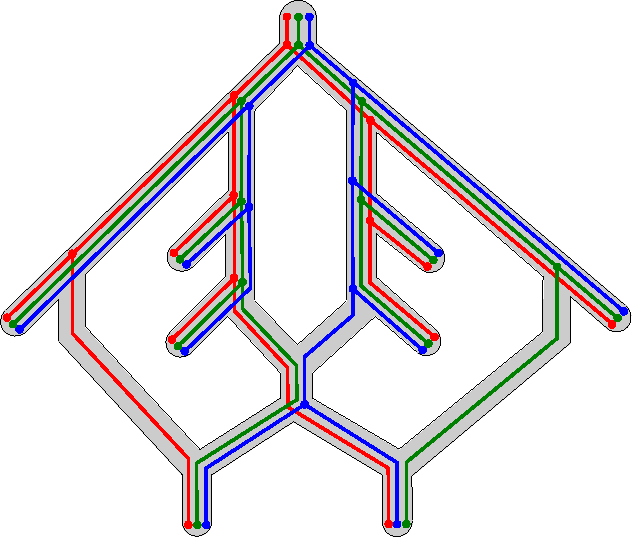
\includegraphics{../figs/ch1/introfig.pdf}
%     \caption{Network displaying three trees, red green and blue.}
%     \label{fig:intronet}
%   \end{figure}
%   %-----------------------------------------------------------------------------

{
A reader interested in the topic of phylogenetic networks, concepts and models that emerge in this area and their applications, is referred to 
\cite{HRS2011,surveycombinatorial2011,Nakhleh2009ProbSolv,Semple2007}.
}

\subsection*{Agreement Forests}

Let $T_1$ and $T_2$ be two rooted binary phylogenetic $X$-trees. Consider now a set of labels $X\cup\{\rho\}$, where $\rho$ is an additional leaf that we attach to the root of both trees $T_1$ and $T_2$. Or more precisely, since a root of any binary phylogenetic tree has outdegree two and indegree zero, we attach an edge to the root and label its  end by $\rho$. See figure \ref{fig:intromaaf}.


{A partition $\cF=\{\cL_\rho,\cL_1,\cL_2,\ldots,\cL_k\}$ of $X\cup\{\rho\}$ is an {\it agreement forest} for~$T_1$ and~$T_2$ if $\rho\in\cL_\rho$ and the following conditions are satisfied:}
\begin{itemize}
\item[(1)] for all $i\in\{\rho,1,2,\ldots,k\}$, we have $T_1|\cL_i \cong T_2|\cL_i$, and
\item[(2)] the trees in $\{T_1(\cL_i): i\in\{\rho,1,2,\ldots,k\}\}$ and $\{T_2(\cL_i): i\in\{\rho,1,2,\ldots,k\}\}$ are vertex-disjoint subtrees of $T_1$ and $T_2$, respectively.
\end{itemize}
In the definition above, the notation $\cong$ is used to denote a graph isomorphism that preserves leaf-labels.

Note that, even though an agreement forest is formally defined as a partition of the leaves $\cF=\{\cL_\rho,\cL_1,\ldots,\cL_k\}$, it is often useful to see it as a collection of trees $\cF=\{F_{\rho}, F_1,\ldots, F_k\}$ where $F_i=T_1|\cL_i$ (or equivalently $F_i=T_2|\cL_i$) for $i\in\{\rho,1,2,\ldots,k\}$. So, intuitively, an agreement forest for~$T_1$ and~$T_2$ can be seen as a collection of trees that can be obtained from either of~$T_1$ and~$T_2$ by deleting a set of edges and subsequently ``cleaning up'' by deleting unlabeled vertices and suppressing indegree-1 outdegree-1 vertices (see figure~\ref{fig:intromaaf}). Therefore, we often refer to the elements of an agreement forest as \emph{components}. The \emph{size} of an agreement forest~$\cF$ is defined as its number of elements (components) and is denoted by~$|\cF|$. 
{A natural optimization problem arises:}\\


\noindent{\bf Problem:} Maximum Agreement Forest (\maf)\\
\noindent {\bf Instance:} Two rooted binary phylogenetic $X$-trees $T_1$ and $T_2$. \\
\noindent {\bf Solution:} An agreement forest $\cF$ for $T_1$ and $T_2$. \\
\noindent {\bf Objective:} Minimize $|\cF|-1$ \\

%{It is not immediately obvious why we are minimizing the number of components minus one, but we come back to this shortly.}

The characterization of the hybridization number $h(T_1,T_2)$ in terms of agreement forests that we mentioned in the previous section requires an additional condition. Let $\cF=\{\cL_\rho,\cL_1,\cL_2,\ldots,\cL_k\}$ be an agreement forest for $T_1$ and $T_2$. Let $G_{\cF}$ be the directed graph that has vertex set $\cF$ and an edge $(\cL_i,\cL_j)$ if and only if $i\neq j$ and at least one of the two following conditions holds
\begin{itemize}
\item[(1)] the root of $T_1(\cL_i)$ is an ancestor of the root of $T_1(\cL_j)$ in $T_1$;
\item[(2)] the root of $T_2(\cL_i)$ is an ancestor of the root of $T_2(\cL_j)$ in $T_2$.
\end{itemize}
The graph $G_{\cF}$ is called the {\it inheritance graph} associated with $\cF$. We call $\cF$ an {\it acyclic agreement forest} for $T_1$ and $T_2$ if $G_{\cF}$ has no directed cycles. If~$\cF$ contains the smallest number of elements (components) over all acyclic agreement forests for $T_1$ and $T_2$, we say that $\cF$ is a {\it maximum acyclic agreement forest} for $T_1$ and $T_2$. Note that such a forest is called a \emph{maximum} acyclic agreement forest, even though one \emph{minimizes} the number of elements, because in some sense the ``agreement'' is maximized. (Also note that acyclic agreement forests were called \emph{good} agreement forests in~\cite{baroni05}.)

We define $m_a(T_1, T_2)$ to be the number of elements of a maximum acyclic agreement forest for~$T_1$ and~$T_2$ minus one. Also the problem of computing $m_a(T_1, T_2)$ has an optimization counterpart:\\


\noindent{\bf Problem:} Maximum Acyclic Agreement Forest (\maaf)\\
\noindent {\bf Instance:} Two rooted binary phylogenetic $X$-trees $T_1$ and $T_2$. \\
\noindent {\bf Solution:} An acyclic agreement forest $\cF$ for $T_1$ and $T_2$. \\
\noindent {\bf Objective:} Minimize $|\cF|-1$.\\


We minimize $|\cF|-1$, rather than~$|\cF|$, following~\cite{bordewich07a}, because $|\cF|-1$ corresponds to the number of edges one needs to remove from either of the input trees to obtain~$\cF$ (after ``cleaning up'') and because of the relation we describe below between this problem and {\sc MinimumHybridization}. Nevertheless, it can be shown that, from an approximation perspective, it does not matter whether one minimizes~$|\cF|$ or~$|\cF|-1$ (which is not obvious).

\begin{theorem}{\cite[Theorem 2]{baroni05}}\label{t:hybrid}
Let $T_1$ and $T_2$ be two rooted binary phylogenetic $X$-trees. Then
$$h(T_1,T_2)=m_a(T_1,T_2).$$
\end{theorem}


%--------------------------------------------------------------------------
\begin{figure}
    \centering
     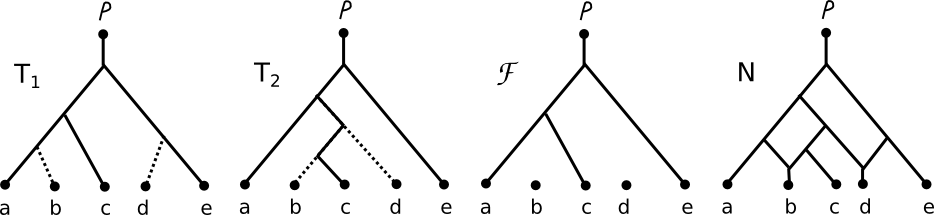
\includegraphics[scale=.5]{../figs/ch1/intromaaf.png}
    \caption{Two phylogenetic trees,~$T_1$ and~$T_2$, an acyclic agreement forest~$\cF$ for~$T_1$ and~$T_2$ with three components and its inheritance graph (which will later be drawn instead of that network). Forest~$\cF$ can be obtained from either of~$T_1$ and~$T_2$ by deleting the dashed edges.} 
    \label{fig:intromaaf}
\end{figure}
%--------------------------------------------------------------------------


 
  %------------------------------------------------------------------------------
  
\section{Related work}
  %------------------------------------------------------------------------------
  

There are many types of problems that arise in the area of phylogenetic networks, but they can all be summarized as having a goal of reconstructing a network from the available data. The variety of problems come (in part) from variety of different kinds of data. In this thesis we mainly look at the problem of constructing a phylogenetic network from trees, but there are also techniques which construct networks from clusters \cite{KelkScornavacca2011, elusiveness}, triplets \cite{kelklev2, simptrip}, quartets \cite{YGXW2014, GBP2012}, networks \cite{IerselMoulton2014, HuberMoulton2013, HIMW2014, 2014arXiv1411.6804H}, sequences \cite{jin2006maximum, JNST2007b, JNST2006a, ParkNakhleh2012b, FischerIKS15} and distances between those sequences \cite{francis2015tree, Willson2013}.



A standard reference book on this topic is \cite{SemSte03}, in which the authors set the mathematical foundations for phylogenetics. A more recent text \cite{DreHub12} focuses on different ways of encoding phylogenetic networks and how they are related to each other. For a more practical flavour there is \cite{HRS2011}. For algorithms on ancestral recombination graphs see \cite{Gusfield2014}.







%\textcolor{magenta}{MIN HYB: 2 BINARY TREES} \textcolor{blue}{ - Complexity, FPT alg}

Most of the problems on constructing a network on available type of data are NP-complete. In this thesis we mainly focus on \mh. The ultimate goal for this problem is to develop algorithms that can cope with many input trees and nonbinary input trees~\cite{davidbook} and to take different causes of incongruence into account, see e.g. \cite{yu2013parsimonious}.  However, until recently most algorithmic research has focused on the simplest possible case: two input trees, both binary. Unfortunately even this version of the problem is NP-hard and APX-hard \cite{bordewich07a}.


Fortunately the binary two-tree problem is fixed parameter tractable. In \cite{bordewich07b}, Bordewich and Semple proved that \mh for two rooted binary trees is FPT and gave an algorithm with running time $O((28k)^k + n^3)$. This result was established via kernelization - a common technique in parameterized complexity where one wants to prove that a kernel, bounded in size as a function of some parameter, can be found in polynomial time. The theoretical state of the art is an algorithm based on bounded-search with running time $\Oh(3.18^k n)$ \cite{whidden2013fixed} with~$n=|X|$ and $k$ the reticulation number. 

A standard approach in the network literature is to look for algorithms parameterized by the number of reticulations of an optimal network. On this front, a variety of increasingly sophisticated algorithms have been developed \cite{bordewich2,bordewich07b,hybridnet,quantifyingreticulation,firststeps,whiddenFixed,whiddenWABI}. These show that for many practical instances of \mh the problem can be efficiently solved.


In the nonbinary setting, \mh is of course NP-hard and APX-hard. While there do exist efficient FPT algorithms for the binary variant of the problem, the nonbinary variant of the problem has received comparatively little attention, although that too is FPT \cite{linzsemple2009,teresaFPT}. In both of these results, the practical applicability of the FPT algorithms is limited to instances of small or moderate size, for larger instances approximation algorithms are required. An example of an approach via kernalization is \cite{IerselKelk2014} where the authors give two algorithms for \mh on multiple nonbinary trees. 

%\cite{vanIerselLinz} where van Iersel and Linz give a quadratic size kernel for \mh on multiple binary phylogenetic trees, while in 




 

% \textcolor{magenta}{MAAF} \textcolor{blue}{}
% 
% 
% The MAAF abstraction gives a useful static characterization of the two-tree hybridization number problem \cite{bordewich07a}. In particular, in the two-tree case the MAAF abstraction essentially allows us to bypass the problem of actually constructing the hybridization network: it can easily be constructed  in polynomial time from the components of the MAAF.  This abstraction, and related FPT results, also hold in the case of two \emph{non}binary trees, albeit with significant technical complications \cite{linzsemple2009,teresaFPT}. 
% 
% For computing all \maaf we have an algorithm from Chen and Wang given in  \cite{chen2012algorithms}.




In the last chapter of this thesis we look at quite a different problem. There we are given unrooted trees, not always on the same set of taxa, and the questions is weather there exists a supertree that displays all the partial trees. When such a tree exists we say that the instance is compatible. Even though this is an NP hard problem, it is fixed parameter tractable \cite{BryLag06}. That result is purely theoretic and no practical FPT algorithm is known. There exists however a number of useful characterizations. 

There is a well known characterization of compatibility of undirected multi-state characters \cite{Buneman1974205}, and many other authors have since found interesting characterizations in terms of chordal graphs \cite{gysel2012reducing, meacham1983, Semple2002169}. As a counterpart to Buneman's triangulation based characterization of undirected multi-state characters \cite{Buneman1974205}, Vakati and Fern\'andez-Baca \cite{vakati2011graph} gave a triangulation based characterization of the compatibility of unrooted phylogenetic trees in terms of the existence of a specific kind of triangulation in a structure known as the display graph. In \cite{VakBac13} the same authors characterize compatibility of unrooted trees as a chordal graph sandwich problem in a edge label intersection graph, while in \cite{GruHum08} authors define a quartet graph and give a characterization in terms of edge coloring.

Similar work on unrooted trees, but then with a goal of constructing an unrooted network that contains the input trees rather than solving the compatibility problem, was done by Gambette, Berry and Paul. In \cite{GBP2012} for example they show how to adapt some of the well known results on constructing rooted network from triplets on constructing unrooted networks from quartets. In \cite{JRudi2014} the authors give a polynomial time algorithm but then with a restriction on the output: they construct level-1 networks from quartets. 

Finally, building on the idea from \cite{BryLag06}, the authors in \cite{KelkIS15} show the power of monadic second order logic applied to phylogenetics. They observe that many (otherwise NP-hard to compute) measures of (dis)similarity of phylogenetic trees can be bounded and translated (via agreement forests) to a bounded display graph, which then leads to fixed parameter tractability. 




  %------------------------------------------------------------------------------

  
  
\section{Structure of the thesis and contribution}

We start with an approximability result in Chapter \ref{ch:1}. There we show that the problem \mh has a constant factor polynomial-time approximation if and only if the problem of computing a minimum-size feedback vertex set in a directed graph (\dfvs) has a constant factor polynomial-time approximation. Despite considerable attention from the combinatorial optimization community, it remains to this day unknown whether such an algorithm exists for \dfvs. The proof of this result leads to a new insight into where the hardness of the problem lies, and based on this we develop a practically efficient algorithm in Chapter \ref{ch:2} and give its generalization to biologically more relevant situations in Chapter~\ref{ch:3}. 

Chapter \ref{ch:1} is based on the paper \textit{Cycle killer...qu'est-ce que c'est? On the comparative approximability of hybridization number and directed feedback vertex set}. It was written together with Steven Kelk, Leo van Iersel, Simone Linz, Celine Scornavacca and Leen Stougie in 2011. It is published in SIAM Journal on Discrete Mathematics. The follow-up paper written with Leo van Iersel, Steven Kelk and Celine Scornavacca, \textit{A practical approximation algorithm for solving massive instances of hybridization number for binary and nonbinary trees} was first presented at WABI conference in 2012 and later published in BMC Bioinformatics. This is given in Chapter~\ref{ch:2}.

Chapter \ref{ch:3} is based on the third paper in the Cycle Killer series, \textit{Approximation algorithms for nonbinary agreement forests}, coauthored with Leo van Iersel, Steven Kelk and Leen Stougie, published in SIAM Journal on Discrete Mathematics. This paper (and the corresponding chapter) are a little bit more than just a generalization of the previous work to nonbinary trees. We also consider the nonbinary version of problem \maf and give two algorithms for it: an approximation and a parameterized exact algorithm.

In Chapter \ref{ch:4} we consider the same problem, \mh, but now with three binary input trees. Considering three instead of two trees is challenging because the similarity with \maaf weakens and all algorithms for two trees relied on it. Furhermore, all previous algorithms for the multiple tree hybridization problem relied on a brute force search through all possible underlying network topologies, leading to (theoretically unpleasant) running times with towers of exponents (i.e. not $O(c^k poly(n))$ for any $c$). We improve that by giving a $O(c^k poly(n))$ running time. This chapter is based on paper currently under review, \textit{Hybridization Number on Three Trees}, written with Leo van Iersel, Steven Kelk, Chris Whidden and Norbert Zeh.

Chapter \ref{ch:5} has quite a different flavor than the rest of the thesis. Though still phylogenetically motivated, we turn our attention to unrooted trees. Here the goal is to puzzle the partial unrooted trees together into a single tree that contains all the topologies of the partial trees. We build on work of Bryant and Lagergren \cite{BryLag06} and give a condition for when the partial trees do belong to a single larger tree. This work was done together with Alexandar Grigoriev and Steven Kelk and published in Journal of Graph Algorithms and Applications. It was also presented at AlCoB conference in 2014. 






%Despite considerable attention from the combinatorial optimization community, it remains to this day unknown whether a constant factor polynomial-time approximation exists for DFVS. 

%Our result thus places the (in)approximability of hybridization number in a much broader complexity context, and as a consequence we obtain that it inherits inapproximability results from the problem Vertex Cover. On the positive side, we use results from the DFVS literature to give an $\text{O}( \log r \log \log r)$ approximation for the hybridization number if $r$ is the correct value.

%In the previous chapter we showed how, for the binary variant of \maaf, large instances \emph{can} however be very well approximated using a specific marriage of \maf and \dfvs solvers. This approach is exponential-time in the worst case but in practice is very fast and yields highly competitive approximation factors. 







